%% Modified LaTeX-Beamer template, stolen from the SDQ group and
%% adapted by Philipp Becker
%% Original Statement:

%%------------------------------------------------------------
%% LaTeX-Beamer template for KIT design
%% by Erik Burger, Christian Hammer
%% title picture by Klaus Krogmann
%%
%% version 2.5
%%
%% mostly compatible to KIT corporate design v2.0
%% http://intranet.kit.edu/gestaltungsrichtlinien.php
%%
%% Problems, bugs and comments to
%% burger@kit.edu
%%------------------------------------------------------------
%% Class options
%%   aspect ratio options:
%%   -- 16:9 (default)
%%   -- 4:3
%%   language options:
%%   -- en (default)
%%   -- de
%%   position of navigation bar:
%%   -- navbarinline (default): bottom of the white canvas
%%   -- navbarinfooter : more compressed variant inside the footer
%%   -- navbarside : side bar at the left of the white canvas
%%   -- navbaroff : none
%% example: \documentclass[16:9,de,navbarinfooter]{sdqbeamer}

\documentclass[navbaroff]{sdqbeamer}

%% TITLE PICTURE

% if a custom picture is to be used on the title page, copy it into the 'logos'
% directory, in the line below, replace 'myimage' with the
% filename (without extension) and uncomment the following line
% (picture proportions: 63 : 20 for standard, 169 : 40 for wide
% *.eps format if you use latex+dvips+ps2pdf,
% *.jpg/*.png/*.pdf if you use pdflatex)

% \titleimage{myimage}

%% GROUP LOGO

% for a custom group logo, copy your file into the 'logos'
% directory, insert the filename in the line below and uncomment it

% \grouplogo{mylogo}

% (*.eps format if you use latex+dvips+ps2pdf,
% *.jpg/*.png/*.pdf if you use pdflatex)

%% GROUP NAME

% for groups other than SDQ, please insert in the line below and uncomment it
% \groupname{My group}

% the presentation starts here

\title[Safe RL for Robot Navigation with MPC]{Safe Reinforcement Learning for Robot Navigation \\ with Model Predictive Control}
\subtitle{PhD Defense, Jury: Alian Dutech, Nicolas Mansard, Laetitia Matignon, Olivier Aycard, Pierre-Brice Wieber, Thierry Fraichard}
\author{ Dhimiter Pikuli}

% Bibliography

% \usepackage[citestyle=authoryear,bibstyle=numeric,hyperref,backend=biber]{biblatex}
\usepackage{color,colortbl}
\usepackage{xcolor}
\usepackage{multirow}
\usepackage{multicol}
\usepackage{verbatim}
\usepackage{Styles/mymath}

% \addbibresource{presentation.bib}
% \bibhang1em

\begin{document}

%title page
\KITtitleframe

\newcommand\Fontvi{\fontsize{15}{15}\selectfont}
\newcommand\Fontvii{\fontsize{9}{7}\selectfont}
\newcommand\Fontviii{\fontsize{7}{4}\selectfont}
\newcommand\Fontviiii{\fontsize{12}{12}\selectfont}
\newcommand\Fontbig{\fontsize{30}{4}\selectfont}
\newcommand\Fontviiiiii{\fontsize{5}{4}\selectfont}
%table of contents

\definecolor{myred}{RGB}{255,108,107}
\definecolor{lightred}{RGB}{255,208,207}
\definecolor{myblue}{RGB}{81,127,255}
\definecolor{lightblue}{RGB}{151,197,255}
\definecolor{mygreen}{RGB}{80,176,123}
\definecolor{lightgreen}{RGB}{130,226,183}
\definecolor{green}{RGB}{51,224,200}
\definecolor{lejla}{RGB}{162,97,255}
\definecolor{orange}{RGB}{210,125,69}

\section{Section 1}
\subsection{Subsection 1.1}
\begin{frame}{}
    \centering
    \textbf{\Fontbig{Introduction}}
\end{frame}

\begin{frame}{Thesis}
    \centering
    \textbf{\Fontviiii{Safe Reinforcement Learning for Robot Navigation with Model Predictive Control}}
    \vspace{4cm}
    \begin{textblock*}{6cm}(0.88cm,2.45cm)
        \begin{tikzpicture}
            \path[use as bounding box] (-1,0) rectangle (15,0.55);
            % Rounded rectangle
            \draw<2->[rounded corners=6pt, ultra thick, mygreen] (5.2,0) rectangle (8.54,0.55);
            \draw<4->[rounded corners=6pt, ultra thick, orange] (0.05,0) rectangle (4.6,0.55);
            \draw<6->[rounded corners=6pt, ultra thick, myblue] (9.42,0) rectangle (14.15,0.55);

            % Arrow from the bottom border pointing down
            \draw<3->[-{Stealth}, ultra thick, mygreen] (6.97,0) -- (6.97,-1.5);
            \draw<5->[-{Stealth}, ultra thick, orange] (2.325,0) -- (2.0,-1.5);
            \draw<7->[-{Stealth}, ultra thick, myblue] (12,0) -- (12,-1.5);

            % Environment
            \node<3->[fill=black!14, minimum width=5cm, minimum height=3cm] (env) at (6.97, -3) {};
            \draw<3->[ultra thick] (4.47, -4) -- (6.97, -1.5);
            \draw<3->[ultra thick, mygreen] (4.47, -4.5) -- (9.47, -4.5) -- (9.47, -1.5) -- (4.47, -1.5) -- cycle;
            \fill<3->[black!5] (4.5, -3.94) -- (6.91, -1.53) -- (4.5, -1.53) -- cycle;
            \node<3->[anchor=west] at ([yshift=-0.5cm]env.center) {
\includegraphics[height=1cm]{imgs/mirokai.png}};
            \node<3->[anchor=center] at ([xshift=-1.1cm]env.center) {
\includegraphics[height=1.2cm]{imgs/walking.png}};
            \node<3->[anchor=east] at ([xshift=2cm]env.center) {\reflectbox{
\includegraphics[height=1.2cm]{imgs/walking.png}}};
            \node<3->[anchor=east] at ([xshift=0.45cm, yshift=0.8cm]env.center) {
\includegraphics[height=1.2cm]{imgs/walking.png}};

            % RL
            \node<5->[draw, ultra thick, orange, fill=black!5, minimum width=4cm, minimum height=3cm] (rl) at (2.0, -3) {};
            \node<5->[xshift=-1.2cm] at (rl.center) {\resizebox{1.2cm}{!}{\begin{tikzpicture}
  % Antenna stalk
  \draw[very thick] (0,2) -- (0,2.7);
  % Antenna ball
  \fill[red!50] (0,3) circle (0.28);
  \draw[thick] (0,3) circle (0.28);

  % Ears
  \draw[thick, rounded corners=2pt, fill=black!8]
        (-2.35,-0.55) rectangle (-1.95,0.55);
  \draw[thick, rounded corners=2pt, fill=black!8]
        (1.95,-0.55) rectangle (2.35,0.55);

  % Head
  \draw[very thick, rounded corners=12pt, fill=blue!15]
        (-2,-2) rectangle (2,2);

  % Eyes (whites)
  \fill[white] (-0.9,0.5) circle (0.45);
  \draw[thick] (-0.9,0.5) circle (0.45);
  \fill[white] (0.9,0.5) circle (0.45);
  \draw[thick] (0.9,0.5) circle (0.45);

  % Pupils
  \fill (-0.88,0.5) circle (0.17);
  \fill (0.88,0.5) circle (0.17);

  % Cheeks
  % \fill[red!35, opacity=0.7] (-1.45,-0.45) circle (0.22);
  % \fill[red!35, opacity=0.7] (1.45,-0.45) circle (0.22);

  % Mouth with teeth
  \draw[very thick, rounded corners=3pt, fill=white]
        (-0.85,-1.35) rectangle (0.85,-0.65);
  \draw[thick] (-0.3,-1.35) -- (-0.3,-0.65);
  \draw[thick] (0.3,-1.35) -- (0.3,-0.65);
  \draw[thick] (-0.85,-1.0) -- (0.85,-1.0);
\end{tikzpicture}
}};
            \node<5->[xshift=1.2cm, yshift=-0.05cm] at (rl.center) {
\includegraphics[height=1.5cm]{imgs/world_.png}};
            \draw<5->[->, ultra thick] (1.4, -2.5) to[bend left=40] (2.6, -2.5);
            \draw<5->[->, ultra thick] (2.6, -3.7) to[bend left=40] (1.4, -3.7);

            % MPC
            \node<7->[draw, ultra thick, myblue, fill=black!5, minimum width=4cm, minimum height=3cm] (mpc) at (12.0, -3) {};
            \node<7->[xshift=-1.2cm] at (mpc.center) {\resizebox{1.4cm}{!}{\begin{tikzpicture}
    % Level curves of the 2D function (nested ellipsoids)
    \draw[thick, blue!60] [rotate around={28:(0,0)}] (0,0) ellipse (4.3 and 2.7);
    \draw[thick, blue!55] [rotate around={33:(0.1,-0.05)}] (0.1,-0.05) ellipse (3.4 and 2.2);
    % \draw[thick, blue!50] [rotate around={25:(-0.08,0.06)}] (-0.08,0.06) ellipse (2.7 and 1.75);
    \draw[thick, blue!45] [rotate around={28:(-0.02,0.08)}] (-0.02,0.08) ellipse (2.35 and 1.55);
    \draw[thick, blue!40] [rotate around={26:(-0.04,-0.06)}] (-0.04,-0.06) ellipse (1.45 and 0.95);
    \draw[thick, blue!35] [rotate around={34:(0.06,-0.04)}] (0.06,-0.04) ellipse (0.9 and 0.6);
    \draw[thick, blue!30] [rotate around={28:(0,0)}] (0,0) ellipse (0.45 and 0.3);

    % Zigzag optimization path converging to the optimum
    \draw[line width=2.2mm, myred]
          (3.6,3) -- (1.8,2.9) -- (2.4,1.4) -- (0.2,1.6) -- (0.9,0.6) -- (-0.7,0.45) -- (-0.25,-0.15) -- (0.02,-0.02);

    % Optimum point
    \fill[myred] (0,0) circle (0.12);

    % Starting point
    \fill[myred] (3.6,3) circle (0.12);
\end{tikzpicture}
}};
            \node<7->[xshift=1.2cm] at (mpc.center) {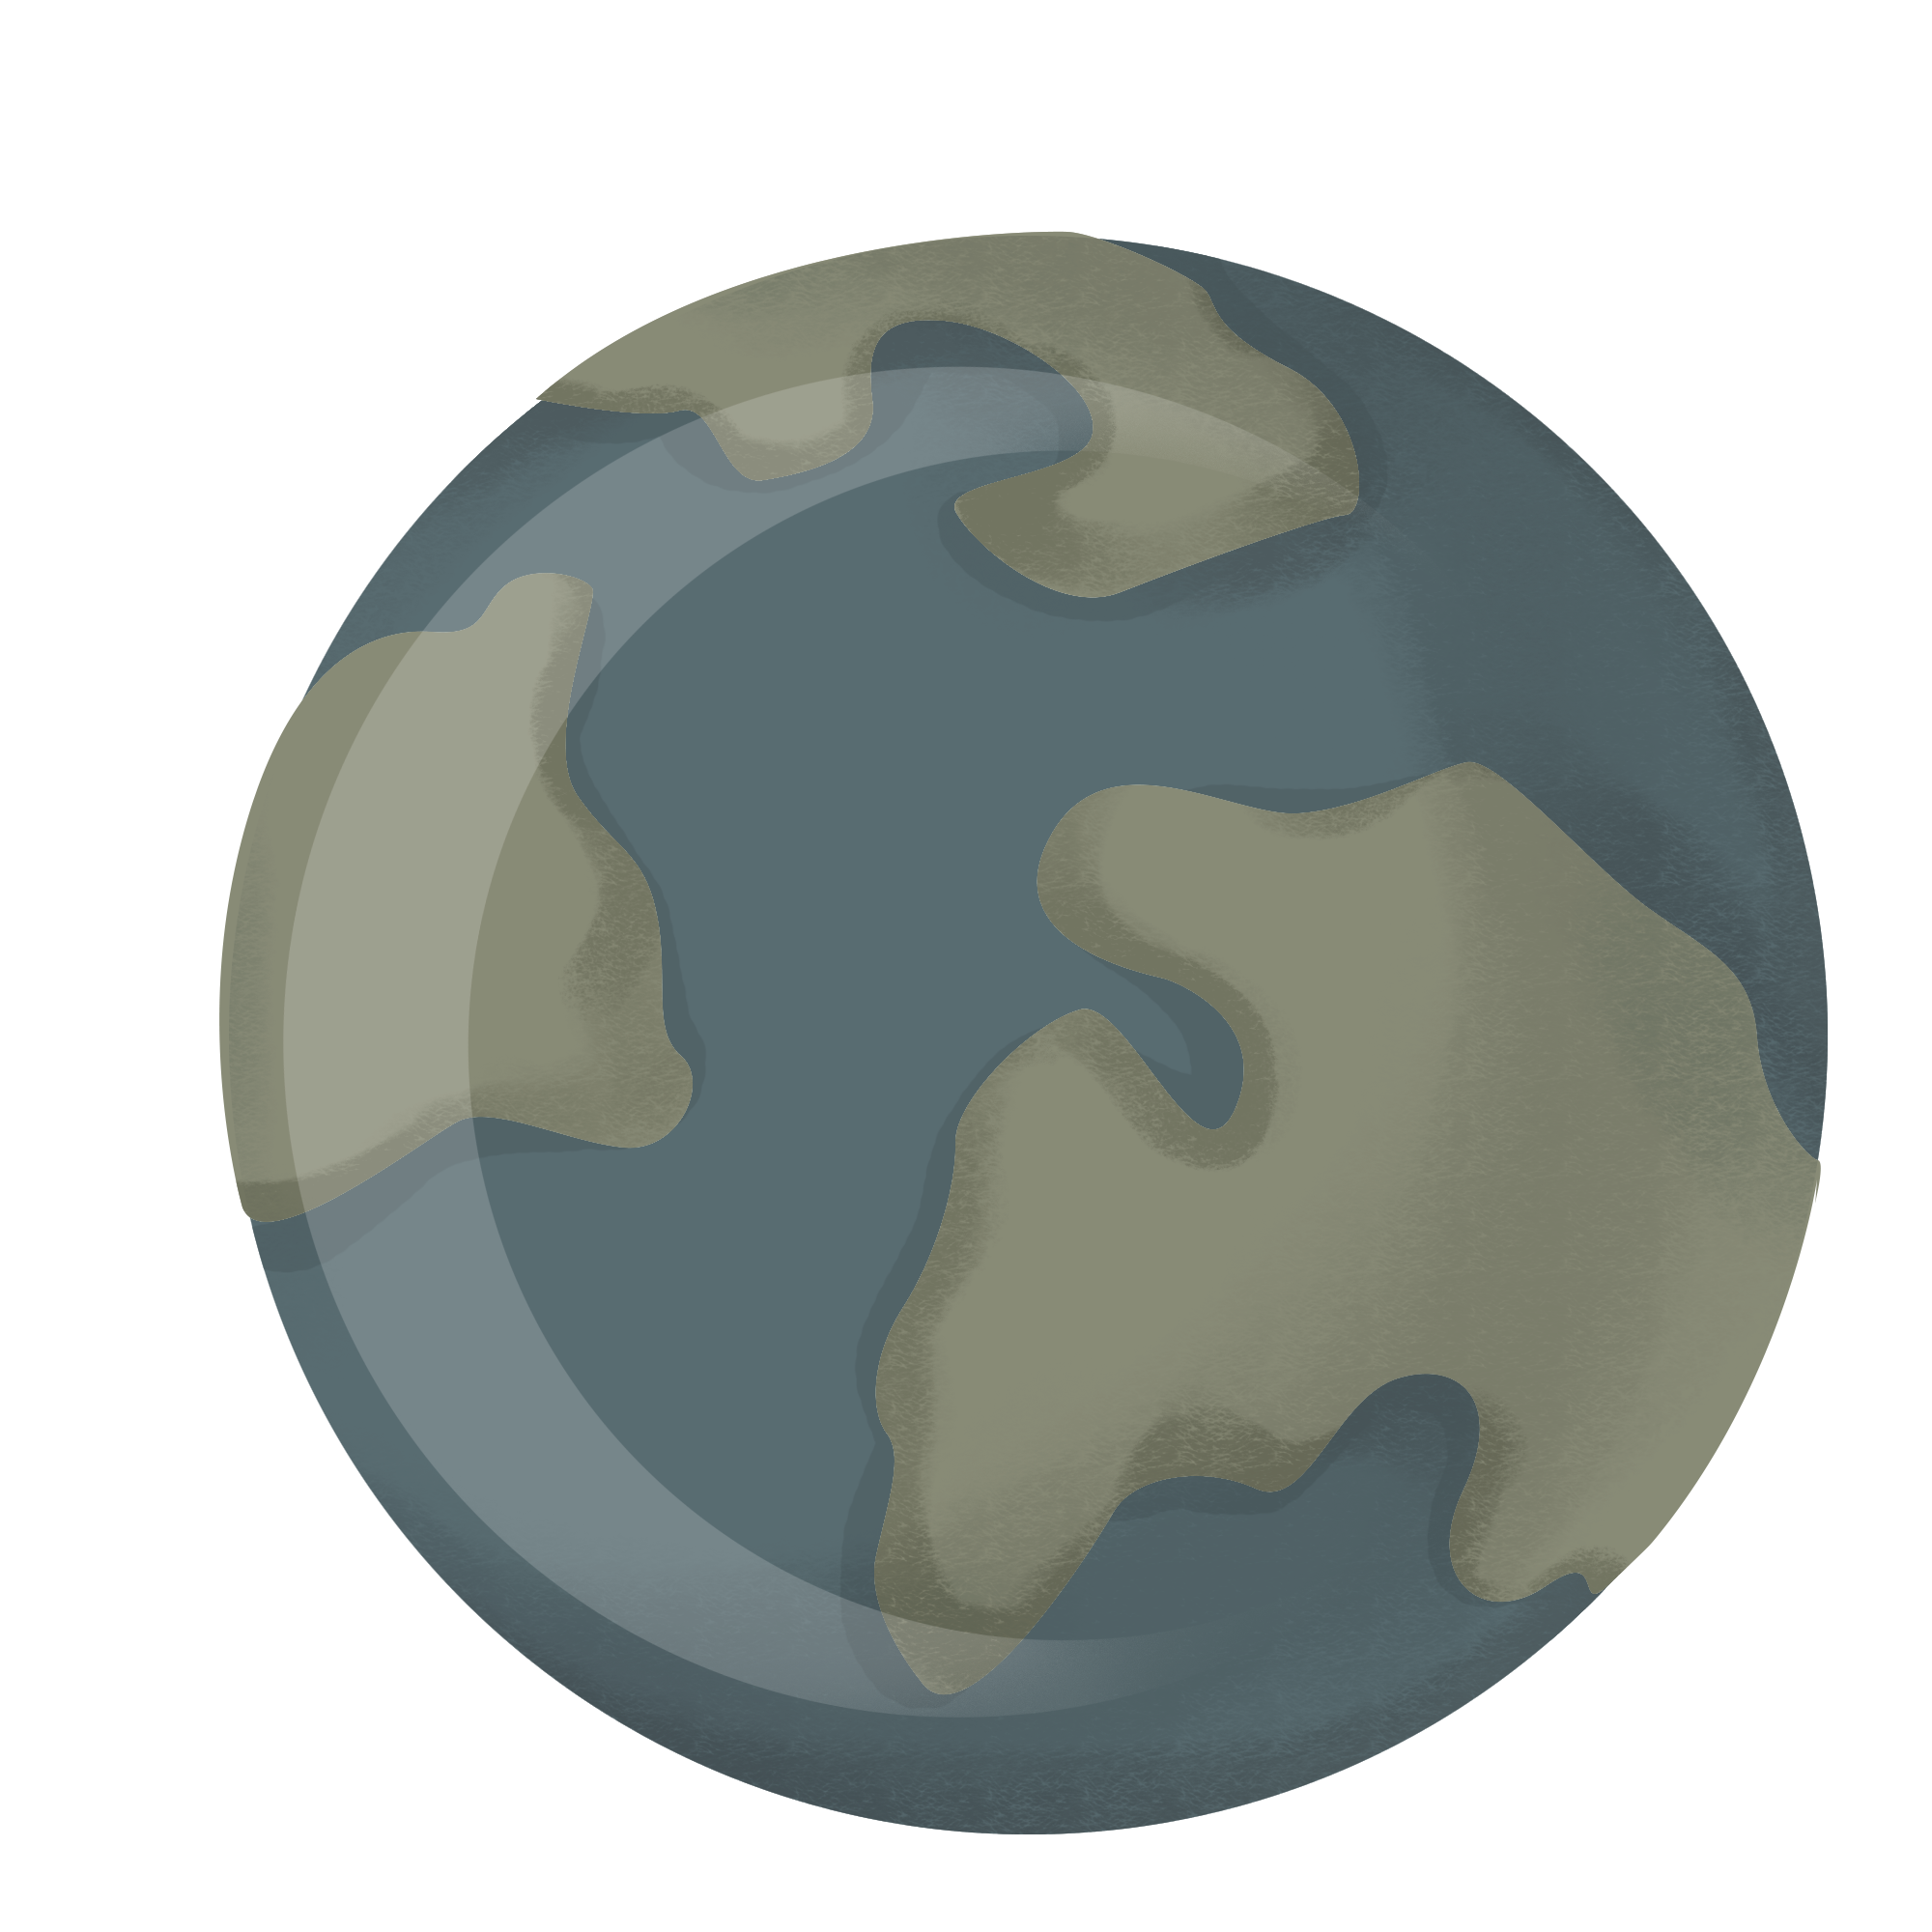
\includegraphics[height=1.2cm]{imgs/world_bw.png}};
            \node<7->[xshift=1.2cm, yshift=0.9cm] at (mpc.center){
                \begin{tikzpicture}[scale=0.1]
                    \draw[->, black!30] (-2.8,0) -- (2.8,0);
                    \draw[->, black!30] (0,-0.3) -- (0,5);
                    \draw[very thick, myred, domain=-3:3, smooth] plot (\x, {0.6*\x*\x});
                \end{tikzpicture}
            };
            \node<7->[xshift=1.2cm, yshift=-1cm] at (mpc.center){
                \begin{tikzpicture}[scale=0.1]
                    \draw[->, black!30] (-2.8,0) -- (2.8,0);
                    \draw[->, black!30] (0,-0.3) -- (0,5);
                    \draw[very thick, black, domain=-3:3, smooth] plot (\x, {0.6*\x*\x});
                    \draw[very thick, myred] (-3,1) -- (3,2.2);
                \end{tikzpicture}
            };
            \draw<7->[-{Stealth}, ultra thick] (12.6, -3) -- (11.5, -3);
            \draw<7->[-{Stealth}, ultra thick] (12.6, -2.1) -- (11.45, -2.8);
            \draw<7->[-{Stealth}, ultra thick] (12.6, -4) -- (11.45, -3.2);
            \draw<8->[-{Stealth}, ultra thick] (13.2, -4.35) -- (13.2, -4.8) -| (-0.4,0);
        \end{tikzpicture}
    \end{textblock*}
\end{frame}

% example scope
% \begin{scope}[on above layer]
%     \draw
%         <3->{
%             (const) edge[G] (0, -4.86)
%             (const) edge[G] (1.36, -2)
%             (const) edge[G] (2.5, -2.2)
%             (const) edge[G] (3.06, -1.4)};
%     \draw
%         <2->{(traj) edge[L] (3.5, -2.8)};
%     \end{scope}

\subsection{Subsection 1.2}
\begin{frame}{Context}
    \begin{itemize}
        \item Inria + UGA + MIAI
            \pause
        \item Collaborators: KIT and Enchanted Tools
            \pause
        \item Background\\
            Inria: safe robot control\\
            KIT: learning for robot control\\
            Enchanted Tools: Mirokai robot
            \pause
        \item Thesis focus: \textbf{safe \& efficient robot navigation}
        \item Another thesis for social navigation (Jordan Cosio)
    \end{itemize}
        \begin{textblock*}{10cm}(9.5cm,2.2cm)
            
\includegraphics[width=2cm]{imgs/logo_inria.png}\hspace{0.4cm}
            \raisebox{-3mm}{
\includegraphics[width=2cm]{imgs/Logo_UGA.png}\hspace{0.4cm}}
            
\includegraphics[width=2cm]{imgs/logo_miai.png}
        \end{textblock*}
    \only<2->{
        \begin{textblock*}{10cm}(9.5cm,3.8cm)
            
\includegraphics[width=2cm]{imgs/Logo_KIT.png}\hspace{0.4cm}
            \includegraphics[width=2cm]{imgs/alr-logo.png}\hspace{0.4cm}
            
\includegraphics[width=2cm]{imgs/Enchanted_Tools_Logo.png}
        \end{textblock*}
    }
\end{frame}

\subsection{Subsection 1.3}
\begin{frame}{Robot Crowd Navigation}
    \begin{itemize}
        \item Goal\\
            \pause
            - reach the assigned goal\\
            \pause
            - avoid the crowd \\
            \pause
            - non-verbal cooperation\\
            \pause
            - our scope is local navigation
            % without communicating, perception, self-localizing, planning, map building
        \pause
    \vspace{4mm}
    \item Formalization \\
        $\rightarrow$ Markov Decision Process (MDP)\\
        \pause
        - $(\mathcal{S,A,P,R})$\\
        \pause
        - $\mathcal{S}=\{\V{s}_1, \V{s}_2, \V{s}_3\}$\\
        \pause
        - $\mathcal{A}=\{\textcolor{myblue}{\V{a}_1}, \textcolor{myred}{\V{a}_2}\}$\\
        \pause
        - $\mathcal{R}:\mathcal{S}\times\mathcal{S}\times\mathcal{A}\rightarrow\mathbb{R}$\\
            $\;\;\equiv\{(\V{s}_1,\V{s}_2,\V{a}_2)\rightarrow 1, (\V{s}_3,\V{s}_3,\V{a}_1)\rightarrow 5 \dots\}$\\
        \pause
        - $\mathcal{P}:\mathcal{S}\times\mathcal{S}\times\mathcal{A}\rightarrow \left[0, 1\right] $
    \end{itemize}
    \begin{textblock*}{4.8cm}(6.2cm,1.8cm)
        \visible<1->{
            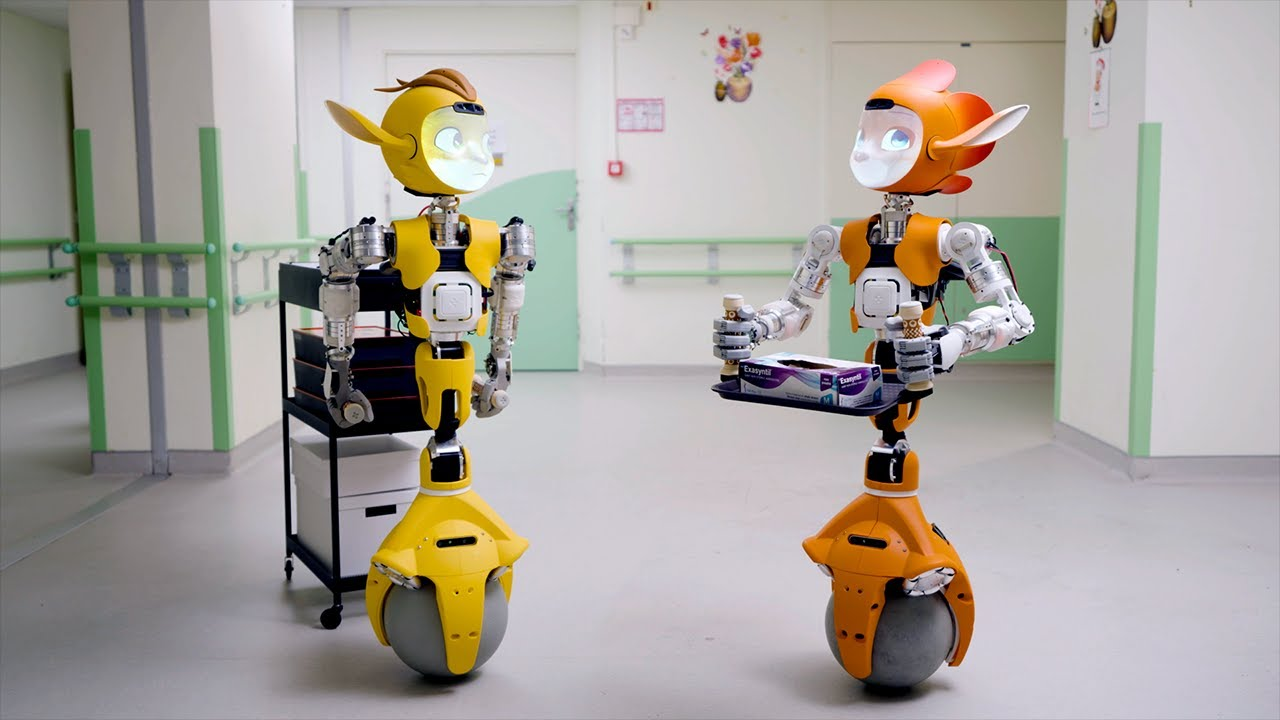
\includegraphics[width=4.8cm]{imgs/miroki.jpg}
            \vspace{-0.7cm}
            \center \Fontviii Mirokai robots from Enchanted Tools
        }
    \end{textblock*}
    \begin{textblock*}{4.8cm}(11.2cm,1.8cm)
        \begin{tikzpicture}
            \node[fill=gray!24, minimum width=5cm, minimum height=3cm] (env) at (6.97, -3) {};
            \draw[ultra thick] (4.47, -4) -- (6.97, -1.5);
            \draw[ultra thick, mygreen] (8.2, -1.8) -- (8.4, -2); % goal
            \draw[ultra thick, mygreen] (8.1, -2.05) -- (8.5, -1.75); % goal
            \draw<2->[->, ultra thick, mygreen] ([xshift=6mm, yshift=-7mm]env.center) to[bend right=30] (8.3, -2);

            \draw[ultra thick, mygreen] (4.47, -4.5) -- (9.47, -4.5) -- (9.47, -1.5) -- (4.47, -1.5) -- cycle;
            \fill[gray!15] (4.5, -3.94) -- (6.91, -1.53) -- (4.5, -1.53) -- cycle;
            \node[anchor=west] at ([yshift=-0.5cm]env.center) {
\includegraphics[height=1cm]{imgs/mirokai.png}};
            \node[anchor=center] at ([xshift=-1.1cm]env.center) {
\includegraphics[height=1.2cm]{imgs/walking.png}};
            \node[anchor=east] at ([xshift=2cm]env.center) {\reflectbox{
\includegraphics[height=1.2cm]{imgs/walking.png}}};
            \node[anchor=east] at ([xshift=0.45cm, yshift=0.8cm]env.center) {
\includegraphics[height=1.2cm]{imgs/walking.png}};

            \draw<3->[ultra thick, myred] ([xshift=1mm, yshift=-7mm]env.center) -- ([xshift=-8mm, yshift=-4.5mm]env.center);
            \draw<3->[ultra thick, myred] ([xshift=6mm, yshift=-7.5mm]env.center) -- ([xshift=14mm, yshift=-4mm]env.center);
            \draw<3->[ultra thick, myred] ([xshift=1mm, yshift=-7mm]env.center) -- ([yshift=1mm]env.center);
        \end{tikzpicture}
    \end{textblock*}
    \begin{textblock*}{7.7cm}(8.4cm,5cm)
        \visible<6->{
            \resizebox{7.7cm}{!}{\begin{tikzpicture}[every node/.append style={ultra thick},
    state/.style = {circle, draw=black, fill=white, minimum size=0.9cm},
    L/.style = {draw, black, line width=2, -{stealth[scale=2]}}]

    % three states in a wide, squashed triangle
    \node[state] (s1) at (-3, 0) {$\V{s}_1$};
    \node[state] (s2) at (3, 0) {$\V{s}_2$};
    \node[state] (s3) at (0, 1.4) {$\V{s}_3$};

    % bottom connections: two arcs of different depth
    \draw[L, draw=myred] (s1) to[bend right=40] node[below, pos=0.5] {$0.4\vert {\color{mygreen}+1}$} (s2);
    \draw[L, draw=myred] (s2) to[bend left=15] node[below, pos=0.5] {$0.8\vert {\color{mygreen}-1}$} (s1);

    % left connections: one arc inside, one outside
    \draw[L, draw=myblue] (s1) to[bend right=22] node[above, pos=0.35, sloped] {$0.1\vert {\color{mygreen}+2}$} (s3);
    \draw[L, draw=myred] (s3) to[bend right=22] node[above left, pos=0.5] {$0.19\vert {\color{mygreen}0}$} (s1);

    % right connections: one arc inside, one outside
    \draw[L, draw=myblue] (s2) to[bend left=22] node[above, pos=0.35, sloped] {$0.1\vert {\color{mygreen}+3}$} (s3);
    \draw[L, draw=myred] (s3) to[bend left=22] node[above right, pos=0.5] {$0.8\vert {\color{mygreen}-2}$} (s2);

    % self-loops
    \draw[L, draw=myblue] (s1) edge[loop left] node[left] {$0.5\vert {\color{mygreen}0}$} (s1);
    \draw[L, draw=myred] (s2) edge[loop right] node[right] {$0.1\vert {\color{mygreen}0}$} (s2);
    \draw[L, draw=myblue] (s3) edge[loop above] node[above] {$0.01\vert {\color{mygreen}+5}$} (s3);
\end{tikzpicture}
}
        }
    \end{textblock*}
\end{frame}

\begin{frame}{Model Predictive Control}
    \begin{itemize}
        \item Problem
        \item Pros \& Cons\\
            + safety
    \end{itemize}
\end{frame}

\begin{frame}{Reinforcement Learning}
    \begin{itemize}
        \item Problem
        \item Pros \& Cons\\
            + learn cooperation\\
            + efficient local path-finding\\
            - safety
    \end{itemize}
    \only<2->{
        \begin{textblock*}{4.8cm}(11cm,5.5cm)
            \centering
            \resizebox{4.8cm}{!}{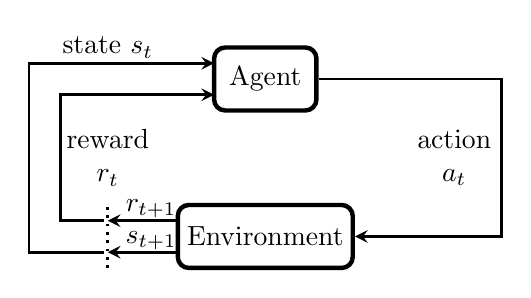
\begin{tikzpicture}[every node/.append style={align=center, ultra thick},
    L/.style = {draw, black, line width=1, -{stealth[scale=2]}},
    G/.style = {draw, black, line width=1}]
    \node[rectangle, minimum height=0.8cm, rounded corners=4pt, minimum width=1.3cm, draw=black] (agent) at (0, 0) {Agent};
    \node[rectangle, minimum height=0.8cm, rounded corners=4pt, minimum width=1.3cm, draw=black] (env) at (0, -2) {Environment};
    \node[] (a) at (2.4, -1) {action \\$a_t$};
    \node[] (s) at (-2, 0.4) {state $s_t$};
    \node[] (r) at (-2, -1) {reward \\$r_t$};
    \node[] (r_) at (-1.45, -1.65) {$r_{t+1}$};
    \node[] (s_) at (-1.45, -2.05) {$s_{t+1}$};
    \draw[->, -{stealth[scale=2]}, black, line width=1] (agent) -| (3, -2) -- (env);
    \draw[->, -{stealth[scale=2]}, black, line width=1] (-2.05, -2.2) -| (-3.0, 0.2) -- (-0.65, 0.2);
    \draw[->, -{stealth[scale=2]}, black, line width=1] (-2.05, -1.8) -| (-2.6, -0.2) -- (-0.65, -0.2);
    \draw
        (-1.1, -2.2) edge[L] (-2, -2.2)
        (-1.1, -1.8) edge[L] (-2, -1.8)
        (-2, -2.4) edge[G, dotted] (-2, -1.6);
\end{tikzpicture}
}
            \vspace{-0.7cm}
            \center \Fontviii RL scheme
        \end{textblock*}
    }
\end{frame}

\begin{frame}{Literature}
    \begin{itemize}
        \item Navigation
        \item Hybrid
    \end{itemize}
\end{frame}

\begin{frame}{Contribution}
    \begin{itemize}
        \item Analysis of freezing behavior for MPC\\
            - MPC analysis\\
            - Cascading
        \item Safe and efficient navigation
            - RL for navigation\\
            - hybrid\\
    \end{itemize}
\end{frame}

\section{Section 2}
\begin{frame}{Reinforcement Learning for Navigation}
\end{frame}

\begin{frame}{Method: RL w/ ProDMP and MPC}
    \begin{itemize}
        \item Dynamic Movement Primitives (DMP)\\
            - $\tau^2\ddot{y}=\alpha(\beta(g-y)-\tau\dot{y})-f$
        \pause
        \item In 2D Navigation $\rightarrow$ 2D trajectories
        \pause
        \item MPC execution and constraints
        \pause
        \item Other considerations\\
            - Predicting crowd movement\\
            - MPC and learning hyperparameters
    \end{itemize}
    % \only<1>{
    %     \begin{textblock*}{6cm}(10.4cm,2.5cm)
    %         \centering
    %         \movie[poster, height=5cm, width=6cm]{}{imgs/primitive.mp4}
    %     \end{textblock*}
    % }
    % \only<2->{
    %     \begin{textblock*}{6cm}(10.4cm,2cm)
    %         \centering
    %         \includegraphics[width=6cm]{imgs/prodmp_mpc.png}
    %     \end{textblock*}
    %     \begin{textblock*}{6cm}(10.4cm,1.4cm)
    %         \begin{tikzpicture}[every node/.append style={rectangle,align=center},
    %             L/.style = {draw, blue, line width=1, -{Stealth[scale=2,length=3,width=3]}},
    %             G/.style = {draw, red, line width=1, -{Stealth[scale=2,length=3,width=3]}},]
    %             \visible<2->{\node[minimum width=1.3cm] (traj) at (3.5, 0) {\Fontviii DMP trajectory};}
    %             \visible<3->{\node[minimum width=1.3cm] (const) at (0, 0) {\Fontviii Crowd Constraints};}
    %             \begin{scope}[on above layer]
    %             \draw
    %                 <3->{
    %                     (const) edge[G] (0, -4.86)
    %                     (const) edge[G] (1.36, -2)
    %                     (const) edge[G] (2.5, -2.2)
    %                     (const) edge[G] (3.06, -1.4)};
    %             \draw
    %                 <2->{(traj) edge[L] (3.5, -2.8)};
    %             \end{scope}
    %         \end{tikzpicture}
    %     \end{textblock*}
    % }
\end{frame}

\section{Section 3}
\begin{frame}{ProDMP MPC}
    \begin{itemize}
        \item MPC\\
            - Debugging and adaptation to parameters\\
            - Uncertainty in the predictions\\
            - FRP (a hacky solution)
        \item ProDMP MPC\\
            - MPC was doing the heavy-lifting\\
            - Entropy too low for TRPL\\
            - Simplifying the problem ($<$ replan)\\
            - Intrinsic Reward
    \end{itemize}
    % \only<1>{
    %     \begin{textblock*}{10cm}(6.5cm,2cm)
    %         $$\dot{\boldsymbol{p}}_{max}=1m/s$$
    %         $$\dot{\boldsymbol{p}}_{c_i,max}=1.5m/s$$
    %         $$\ddot{\boldsymbol{p}}_{max}=10m/s^2$$
    %         $$dt=0.1s$$
    %         $$N=10,20$$
    %     \end{textblock*}
    % }
    % \only<2-9>{
    %     \begin{textblock*}{10cm}(9cm,0.8cm)
    %         \resizebox{8cm}{!}{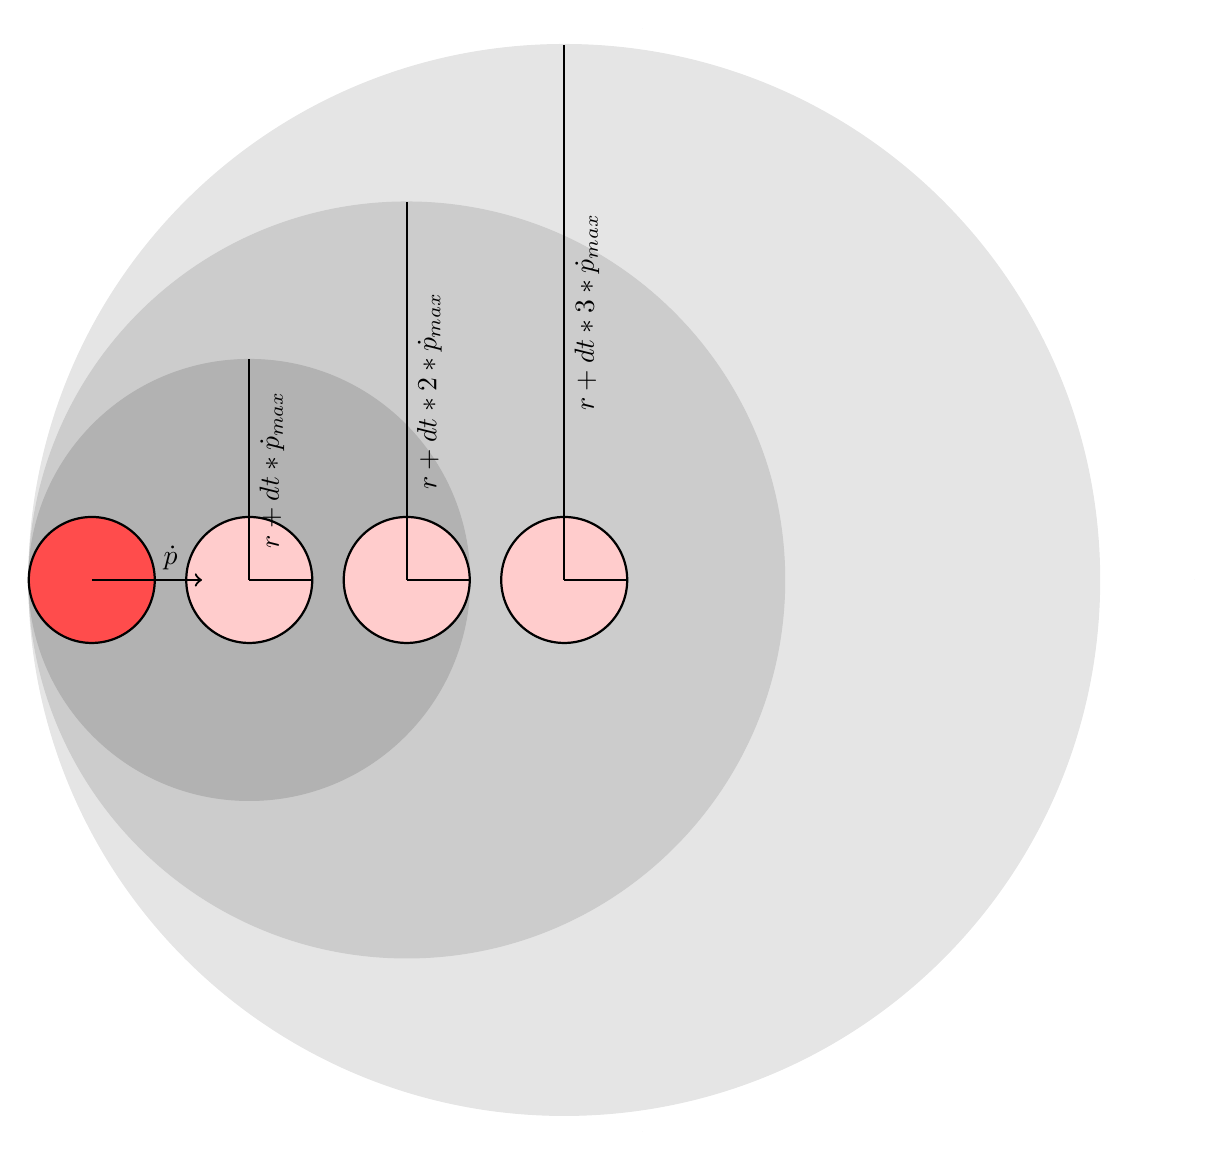
\begin{tikzpicture}
    % Define the centers and radii of the circles
    \coordinate (center1) at (0, 0);
    \coordinate (ref) at (14, 0);
    \coordinate (ref1) at (7, 7);
    \coordinate (ref2) at (7, -7);
    \filldraw[black, thick] (center1) circle(2pt);
    \filldraw[black, thick] (ref) circle(0pt);
    \filldraw[black, thick] (ref1) circle(0pt);
    \filldraw[black, thick] (ref2) circle(0pt);

    % Draw the first circle
    \draw<9->[black!10, fill=black!10] {([xshift=6cm]center1) circle (6.8cm)};
    \draw<8->[black!20, fill=black!20] {([xshift=4cm]center1) circle (4.8cm)};
    \draw<7->[black!30, fill=black!30] {([xshift=2cm]center1) circle (2.8cm)};
    \draw[black, thick, fill=red!70] (center1) circle (0.8cm);
    \draw<4->[fill=red!20, thick] {([xshift=2cm]center1) circle (0.8cm)};
    \draw<5->[fill=red!20, thick] {([xshift=4cm]center1) circle (0.8cm)};
    \draw<6->[fill=red!20, thick] {([xshift=6cm]center1) circle (0.8cm)};
    \draw<3->[->, thick]{(center1) -- ([xshift=1.4cm]center1) node[midway, above, xshift=0.3cm] () {$\dot{\boldsymbol{p}}$}};
    \draw<7->[thick]{
        ([xshift=2cm]center1) -- ([xshift=2cm, yshift=2.8cm]center1) node[midway, below, sloped] () {$r + dt * \dot{\boldsymbol{p}}_{max}$}
        ([xshift=2cm]center1) -- ([xshift=2.8cm]center1)
    };
    \draw<8->[thick]{
        ([xshift=4cm]center1) -- ([xshift=4cm, yshift=4.8cm]center1) node[midway, below, sloped] () {$r + dt * 2 * \dot{\boldsymbol{p}}_{max}$}
        ([xshift=4cm]center1) -- ([xshift=4.8cm]center1)
    };
    \draw<9->[thick]{
        ([xshift=6cm]center1) -- ([xshift=6cm, yshift=6.8cm]center1) node[midway, below, sloped] () {$r + dt * 3 * \dot{\boldsymbol{p}}_{max}$}
        ([xshift=6cm]center1) -- ([xshift=6.8cm]center1)
    };
\end{tikzpicture}
}
    %     \end{textblock*}
    % }
    % \only<10>{
    %     \begin{textblock*}{8cm}(8.5cm,1.4cm)
    %         \begin{figure}[h]
    %             \centering
    %             \includegraphics[width=0.75\textwidth]{imgs/mpc_freeze_s1.png}
    %             \center Predicts a collision in the future, so it freezes
    %         \end{figure}
    %     \end{textblock*}
    % }
    % \only<11>{
    %     \begin{textblock*}{8cm}(8.5cm,1.4cm)
    %         \begin{figure}[h]
    %             \centering
    %             \includegraphics[width=0.75\textwidth]{imgs/mpc_freeze_s2.png}
    %             \center Goal is very close, but constraints still limit behaviour
    %         \end{figure}
    %     \end{textblock*}
    % }
    % \only<12>{
    %     \begin{textblock*}{8cm}(8.5cm,1.4cm)
    %         \begin{figure}[h]
    %             \centering
    %             \includegraphics[width=0.75\textwidth]{imgs/mpc_freeze_s3.png}
    %             \center No goal
    %         \end{figure}
    %     \end{textblock*}
    % }
    % \only<13>{
    %     \begin{textblock*}{8cm}(8.5cm,1.4cm)
    %         \begin{figure}[h]
    %             \centering
    %             \includegraphics[width=0.75\textwidth]{imgs/mpc_freeze_s1.png}
    %             \includegraphics[width=0.75\textwidth]{imgs/mpc_unfreeze_short_horizon.png}
    %             \center Set a shorter horizon in order to ignore collisions far in the future
    %         \end{figure}
    %     \end{textblock*}
    % }
\end{frame}

\begin{frame}{Evaluation}
    \begin{itemize}
        \item Constant moving crowd \&  ORCA
        \pause
        \item SOTA method\\
            - gym-collision-avoidance\\
            - evaluation (`natural' random spawning positions)\\
            - algorithms (GA3C\_CADRL, CADRL, ORCA)
        \pause
        \pause
        \item Reducing the FRP\\
            - comparison of MPC to ProDMP MPC\\
    \end{itemize}
    % \only<2-3>{
    %     \begin{textblock*}{4cm}(9.2cm,1.8cm)
    %         \begin{figure}[h]
    %             \centering
    %             \includegraphics[height=5.4cm]{imgs/GCA_eval_GA3C.png}
    %         \end{figure}
    %         \center \hspace{4mm} GA3C\_CADRL
    %     \end{textblock*}
    % }
    % \only<3>{
    %     \begin{textblock*}{4cm}(13cm,1.8cm)
    %         \begin{figure}[h]
    %             \centering
    %             \includegraphics[height=5.4cm]{imgs/GCA_eval_MPC.png}
    %             \center \hspace{1mm} MPC
    %         \end{figure}
    %     \end{textblock*}
    % }
    % \only<4>{
    %     \begin{textblock*}{7cm}(9.2cm,2.8cm)
    %         \begin{figure}[h]
    %             \centering
    %             \includegraphics[width=1.0\textwidth]{imgs/mpc_freeze_s1.png}
    %             \center Robot freezes because of the constraints in the MPC
    %         \end{figure}
    %     \end{textblock*}
    % }
\end{frame}

\begin{frame}{Metrics}
    \begin{itemize}
        \item Efficiency\\
            - return from the reward function (scalar)\\
            \pause
            - time to goal (seconds)\\
            \pause
            - success rate of reaching goal (percentage)
        \pause
        \item Safety:\\
            - collision rate (percentage)\\
            - collision agent speed ($m/s$)\\
            - collision speed ($m/s$)\\
            \pause
            - collision intersection ($m^2$)
        \pause
        \item FRP\\
            - braking rate (percentage)\\
                MPC will engage in a braking trajectory if the QP solver fails to find a solution
    \end{itemize}
    \only<1-3>{
        \begin{textblock*}{8cm}(8.4cm,2cm)
            \Fontvii
            \begin{align*}
                r_{g} &= \begin{cases}
                    10, & d_t^g < \tau_{\textsc{p}} \land \|\dot{\boldsymbol{p}}\| < a_{\textsc{max}}T, \\
                    C_g(d_{t-1}^g-d_t^g)\vert d_{t-1}^g-d_t^g\vert, & \text{otherwise},
                \end{cases}\\
                r_{c_i} &= \begin{cases}
                    0, & d_{c_i} > \tau_{\textsc{s}}, \\
                    -10, & d_{c_i} < 2\tau_{\textsc{p}}, \\
                    1 - \exp(C_c/d_{c_i}), & \text{otherwise},
                \end{cases}\\
                &\text{where} \; d_t^g =\vert\vert \boldsymbol{p}_t - \boldsymbol{g}\vert\vert, \quad
                 \text{and} \; d_t^{c_i} =\vert\vert \boldsymbol{p}_t - \boldsymbol{p}_{c_i}\vert\vert\\
            \end{align*}
        \end{textblock*}
    }
    \only<2-3>{
        \begin{textblock*}{8cm}(8.4cm,5cm)
            \begin{figure}[h]
                \centering
                \includegraphics[width=8cm]{imgs/ttg.png}
            \end{figure}
            \center \hspace{4mm} Time to goal
        \end{textblock*}
    }
    % \only<4-5>{
    %     \begin{textblock*}{8cm}(9.2cm,1.3cm)
    %         \centering
    %         \resizebox{6cm}{!}{\begin{tikzpicture}
    % Define the centers and radii of the circles
    \coordinate (center1) at (0, 0);
    \coordinate (center2) at (3.5, -4.36);
    \filldraw[blue, thick] (center1) circle(2pt);
    \filldraw[red, thick] (center2) circle(2pt);

    % Draw the first circle
    \draw[name path=circle1, blue!20, thick] ([yshift=-1cm]center1) circle (3cm);
    \draw[name path=circle1, blue!20, thick] ([yshift=-2cm]center1) circle (3cm);
    \draw[name path=circle1, blue!20, thick] ([yshift=-3cm]center1) circle (3cm);
    \draw[blue, ->, thick] (center1) -- ([yshift=-1cm]center1) node[midway, right] () {$\dot{\vec{p}}$} ;

    % Draw the second circle
    \draw[name path=circle2, red!20, thick] ([yshift=2cm]center2) circle (2.6cm);
    \draw[name path=circle2, red!20, thick] ([yshift=4cm]center2) circle (2.6cm);
    \draw[name path=circle2, red!20, thick] ([yshift=6cm]center2) circle (2.6cm);
    \draw[red, ->, thick] (center2) -- ([yshift=2cm]center2) node[midway, right] () {$\dot{\vec{p}}_{c_i}$} ;
    \draw[name path=circle2, red, thick] (center2) circle (2.6cm);
    \draw[name path=circle1, blue, thick] (center1) circle (3cm);
\end{tikzpicture}
}
    %         \vspace{-0.7cm}
    %     \end{textblock*}
    % }
    % \only<5>{
    %     \begin{textblock*}{8cm}(4cm,5.2cm)
    %         \centering
    %         \resizebox{4cm}{!}{\begin{tikzpicture}
    % Define the centers and radii of the circles
    \coordinate (center1) at (0, 0);
    \coordinate (center2) at (3.5, 0);
    \filldraw[blue] (center1) circle(2pt);
    \filldraw[red] (center2) circle(2pt);

    % Draw the first circle
    \draw[name path=circle1, blue, thick] (center1) circle (3cm);

    % Draw the second circle
    \draw[name path=circle2, red, thick] (center2) circle (2.6cm);


    \path[name intersections={of=circle1 and circle2, name=intersection}];

    \fill[blue!30] plot[smooth] coordinates {
        (intersection-2)
        (intersection-1)
    } arc[radius=3cm, start angle=46.2,end angle=-46.2];
    \fill[red!30] plot[smooth] coordinates {
        (intersection-2)
        (intersection-1)
    } arc[radius=2.6cm, start angle=-236.5,end angle=-123.5] coordinate (3.5, 0);
    % \draw[blue] (center1) -- (intersection-1) node[midway, above, sloped, blue] () {$r_0$};
    % \draw[red] (center2) -- (intersection-1) node[midway, above, sloped, red] () {$r_1$};

    \draw (center1) -- (center2) node[midway, below, xshift=-1cm] () {d};
    \draw (intersection-1) -- (intersection-2);
    \filldraw (intersection-1) circle(2pt);
    \filldraw (intersection-2) circle(2pt);
\end{tikzpicture}
}
    %         \vspace{-0.7cm}
    %     \end{textblock*}
    % }
    % \only<6>{
    %     \begin{textblock*}{8cm}(8cm,4.6cm)
    %         \begin{align*}
    %             \mathbb{1}_s&= \left\vert\left\vert \dot{\boldsymbol{p}}_{t-i}\right\vert\right\vert < v_{low} \quad  \forall i\in \{0,\dots, T_f\},\\
    %             \mathbb{1}_o&= \left\vert\left\vert \boldsymbol{p}_{t-i} -\boldsymbol{p}_{t-i-1}\right\vert\right\vert < r_p \quad  \forall i\in \{0,\dots, T_f - 1\},\\
    %             \mathbb{1}_a&= \vert\vert \boldsymbol{g} - \boldsymbol{p}_{t}\vert\vert < \vert\vert \boldsymbol{g} - \boldsymbol{p}_{t-T_f}\vert\vert.
    %         \end{align*}
    %     \end{textblock*}
    % }
\end{frame}


\begin{frame}{Results}
    \begin{itemize}
        \item Constant velocity crowd
        \pause
        \pause
        \pause
        \item ORCA crowd
        \pause
        \pause
        \item Comparison to SOTA (GA3C-CADRL)\\
            - Homogeneous crowd\\
            \pause
            - Heterogeneous crowd
    \end{itemize}

% \only<4-5>{
%         \begin{textblock*}{11cm}(5.4cm,1.4cm)
%             \begin{adjustbox}{width=0.8\textwidth}
%             \begin{tabular}{ | c | c | c | c | c | }
%             \hline
%                 \backslashbox[32mm]{Metrics}{Algorithms} & \makecell{SAC} & \makecell{ProDMP} & \makecell{MPC SH} & \makecell{MPC SH \\ $d \pluseq 0.24$} \\
%             \hline
%                 return $\uparrow$ & 1.56 $\pm$ 0.52 & \textcolor{mygreen}{\textbf{6.25}} $\pm$ 0.47  & 3.65 & 4.16 \\
%                 TTG $\downarrow$ (s) & \textcolor{mygreen}{\textbf{6.44}} $\pm$ 0.29 & 8.3 $\pm$ 0.07 & \textcolor{lightgreen}{\textbf{7.46}} & 7.89 \\
%                 success $\uparrow$ (\%) & \textcolor{myred}{\textbf{39.3}} $\pm$ 1.94 & 63.54 $\pm$ 2.09 & 72.7 & \textcolor{mygreen}{\textbf{80.2}} \\
%             \hline
%                 col. $\downarrow$ (\%) & \textcolor{myred}{\textbf{19.6}} $\pm$ 4.38 & \textcolor{myred}{\textbf{12.86}} $\pm$ 1.47  & \textcolor{myred}{\textbf{23.8}} & \textcolor{myred}{\textbf{10.1}} \\
%                 $\vert\vert\dot{p}-\dot{p}_c\vert\vert\downarrow$ (m/s) & \textcolor{myred}{\textbf{1.74}} $\pm$ 0.08 & \textcolor{mygreen}{\textbf{1.06}} $\pm$ 0.04  & \textcolor{mygreen}{\textbf{1.04}} & 1.22 \\
%                 $\vert\vert\dot{p}\vert\vert$ $\downarrow$ (m/s) & \textcolor{myred}{\textbf{0.94}} $\pm$ 0.02 & \textcolor{myred}{\textbf{0.98}} $\pm$ 0.01  & 0.64 & 0.31\\
%                 col. area $\downarrow$ (m$^2$) & 7.89 $\pm$ 0.09 & 7.58 $\pm$ 0.83  & 5.53 & 7.06 \\
%             \hline
%                 braking $\downarrow$ (\%) & - & - & 12.5 & 22.9 \\
%             \hline
%             \end{tabular}
%             \end{adjustbox}

%             \begin{adjustbox}{width=0.7\textwidth}
%             \begin{tabular}{ | c | c | c | c | c | c | }
%             \hline
%                 \backslashbox[32mm]{Metrics}{Algorithms} & \makecell{ProDMP MPC \\ SH} & \makecell{ProDMP MPC \\ SH, $d \pluseq 0.06$} & \makecell{ProDMP MPC \\ uncert, SH} \\
%             \hline
%                 return $\uparrow$ & \textcolor{mygreen}{\textbf{5.95}} $\pm$ 0.47 & \textcolor{mygreen}{\textbf{6.21}} $\pm$ 0.37 & 3.99 $\pm$ 0.22 \\
%                 TTG $\downarrow$ (s) & 8.53 $\pm$ 0.13 & 8.66 $\pm$ 0.13 & 7.94 $\pm$ 0.05 \\
%                 success $\uparrow$ (\%) & 63.3 $\pm$ 2.56 & 62.4 $\pm$ 5.43 & \textcolor{myred}{\textbf{41.18}} $\pm$ 0.82 \\
%             \hline
%                 col. $\downarrow$ (\%) & \textcolor{lightgreen}{\textbf{2.58}} $\pm$ 0.45 & \textcolor{mygreen}{\textbf{1.22}} $\pm$ 0.31 & \textcolor{myred}{\textbf{11.72}} $\pm$ 0.62 \\
%                 $\vert\vert\dot{p}-\dot{p}_c\vert\vert\downarrow$ (m/s) & 1.23 $\pm$ 0.05 & 1.26 $\pm$ 0.07 & 1.26 $\pm$ 0.02 \\
%                 $\vert\vert\dot{p}\vert\vert$ $\downarrow$ (m/s) & \textcolor{myred}{\textbf{0.65}} $\pm$ 0.06 & 0.58 $\pm$ 0.09 & \textcolor{mygreen}{\textbf{0.0}} $\pm$ 0.0 \\
%                 col. area $\downarrow$ (m$^2$) & \textcolor{mygreen}{\textbf{4.57}} $\pm$ 1.71 & 7.4 $\pm$ 1.98 & 5.88 $\pm$ 0.21\\
%             \hline
%                 braking $\downarrow$ (\%) & \textcolor{mygreen}{\textbf{1.52}} $\pm$ 0.26 & \textcolor{mygreen}{\textbf{1.56}} $\pm$ 0.37 & 14. $\pm$ 0.3 \\
%             \hline
%             \end{tabular}
%             \end{adjustbox}

%         \end{textblock*}
%     }

%     \only<6-7>{
%         \begin{textblock*}{11cm}(6.8cm,1.4cm)
%             \begin{adjustbox}{width=0.7\textwidth}
%             \begin{tabular}{ | c | c | c | c | c | c | c | c | c | c | }
%             \hline
%                 \backslashbox[32mm]{Metrics}{Algorithms} & \makecell{GA3C-\\CADRL} & \makecell{MPC SH \\ relax \\ uncert} & \makecell{ProDMP \\ ORCA} & \makecell{ProDMP MPC \\ ORCA, SH} & \makecell{ProDMP MPC \\ ORCA, SH \\ uncert} \\
%             \hline
%                 return $\uparrow$ & \textcolor{mygreen}{\textbf{0.95}} & 0.56 & \textcolor{lightgreen}{\textbf{0.79}} $\pm$ 0.02 & \textcolor{lightgreen}{\textbf{0.79}} $\pm$ 0.02 & 0.37 $\pm$ 0.01 \\
%                 TTG $\downarrow$ (s) & \textcolor{mygreen}{\textbf{7.36}} & 8.73 & 12.48 $\pm$ 0.29 & 12.87 $\pm$ 0.42 & 16.22 $\pm$ 0.16 \\
%                 success $\uparrow$ (\%) & \textcolor{mygreen}{\textbf{99.84}} & \textcolor{lightgreen}{\textbf{97.68}} & 80.1 $\pm$ 2.3 & 80.1 $\pm$ 2.77 & \textcolor{myred}{\textbf{47.38}} $\pm$ 1.3\\
%             \hline
%                 col. $\downarrow$ (\%) & \textcolor{lightgreen}{\textbf{0.04}} & \textcolor{mygreen}{\textbf{0}} & \textcolor{lightgreen}{\textbf{0.22}} $\pm$ 0.13 & \textcolor{mygreen}{\textbf{0}} & \textcolor{mygreen}{\textbf{0}} \\
%                 $\vert\vert\dot{p} - \dot{p_c}\vert\vert$ $\downarrow$ (m/s) & \textcolor{myred}{\textbf{1}} & \textcolor{mygreen}{\textbf{0}} & \textcolor{myred}{\textbf{0.81}} $\pm$ 0.06 & \textcolor{mygreen}{\textbf{0}} & \textcolor{mygreen}{\textbf{0}}\\
%                 $\vert\vert\dot{p}\vert\vert$ $\downarrow$ (m/s) & \textcolor{myred}{\textbf{1}} & \textcolor{mygreen}{\textbf{0}} & \textcolor{myred}{\textbf{0.94}} $\pm$ 0.03 & \textcolor{mygreen}{\textbf{0}} & \textcolor{mygreen}{\textbf{0}} \\
%             \hline
%                 braking $\downarrow$ (\%) & - & 33.46 & - & \textcolor{mygreen}{\textbf{0.01}} $\pm$ 0 & 2.78 $\pm$ 1.07\\
%             \hline
%             \end{tabular}
%             \end{adjustbox}
%         \end{textblock*}
%     }

%     \only<7>{
%         \begin{textblock*}{11cm}(6.8cm,5cm)
%             \begin{adjustbox}{width=0.7\textwidth}
%             \begin{tabular}{ | c | c | c | c | c | c | c | }
%             \hline
%                 \backslashbox[32mm]{Metrics}{Algorithms} & \makecell{GA3C-\\CADRL} & \makecell{SAC} & \makecell{ORCA} & \makecell{MPC SH \\ relax \\ uncert} & \makecell{ProDMP MPC \\ ORCA, SH} \\
%             \hline
%                 return $\uparrow$ & 0.24 & 0.29 & \textcolor{myred}{\textbf{-0.58}} & 0. &  \textcolor{mygreen}{\textbf{0.56}} \\
%                 TTG $\downarrow$ (s) &  \textcolor{mygreen}{\textbf{7.9}} & 9.01 & \textcolor{lightgreen}{\textbf{8.25}} & 10 &  \textcolor{myred}{\textbf{15.18}} \\
%                 success $\uparrow$ (\%) &  \textcolor{mygreen}{\textbf{97.53}} & 87.73 &  \textcolor{lightgreen}{\textbf{94.93}} &  \textcolor{lightgreen}{\textbf{94.3}} & \textcolor{myred}{\textbf{66.6}} \\
%             \hline
%                 col. $\downarrow$ (\%) &  \textcolor{lightgreen}{\textbf{2}} & \textcolor{myred}{\textbf{9.3}} &  \textcolor{myred}{\textbf{4.5}} &  \textcolor{lightgreen}{\textbf{1.4}} & \textcolor{mygreen}{\textbf{0.27}} \\
%                 $\vert\vert\dot{p} - \dot{p_c}\vert\vert$ $\downarrow$ (m/s) & 0.96 & 1.11 & 1.04 & 1.1 & \textcolor{mygreen}{\textbf{0.91}} \\
%                 $\vert\vert\dot{p}\vert\vert$ $\downarrow$ (m/s) & \textcolor{myred}{\textbf{0.7}} & \textcolor{myred}{\textbf{0.95}} & 0.39 & \textcolor{mygreen}{\textbf{0.35}} & \textcolor{mygreen}{\textbf{0.31}} \\
%             \hline
%                 braking $\downarrow$ (\%) & - & - & - & 23.8 & \textcolor{mygreen}{\textbf{1.2}} \\
%             \hline
%             \end{tabular}
%             \end{adjustbox}
%         \end{textblock*}
%     }
% \end{frame}

% % \begin{frame}{Literature}
% %     \begin{itemize}
% %         \item Revision of SOTA with focus on combining MPC and RL
% %         \pause
% %         \item Crowd simulation and modeling
% %         \pause
% %         \item Freezing Robot Problem (FRP)
% %         \pause
% %         \item Social aspects of navigation
% %         \pause
% %         \item Transformers for RL
% %     \end{itemize}
% % \end{frame}

% \begin{frame}{Cascading MPC}
%     \begin{itemize}
%         \item Decoupling planning and safety
%         \pause
%         \item Two horizons ($M$ and $N$)
%         \pause
%         \item Similar behaviour to MPC
%         \item Short planning and long safety horizon\\
%             - computational cost\\
%             - analysis
%     \end{itemize}
%     \only<1-2>{
%         \begin{textblock*}{10cm}(7cm,2cm)
%             \resizebox{10cm}{!}{\begin{tikzpicture}
    \coordinate (A) at (0, 0);
    \coordinate (mid) at (4, -1);
    \coordinate (B) at (8, 2);
    \node [fill=mygreen, circle, minimum size=0.8cm] at (A) {};
    \node [cross out, ultra thick, draw=mygreen, minimum size=0.4cm, rotate=6] at (B) {};

    \draw[ultra thick, name path=traj] (A) to[out=50,in=130] (mid);
    \draw[ultra thick, -{Stealth[scale=1.4]}, name path=snd_traj] (mid) to[out=-50,in=100] (B);

    \path[name path=inter] (4, -2) -- (4, 4);
    \path[name path=inter_] (1.4, -1) -- (1.4, 2);
    \path[name path=inter__] (6.6, 1) -- (6.6, 2);
    \path[name path=inter___] (8, 1) -- (8, 3);
    \fill [name intersections={of=inter and traj}, draw=myred, fill=myred](intersection-1) circle (2pt) node[below left] {$i=2, j=1$};
    \fill [name intersections={of=inter_ and traj}, draw=myred, fill=myred](intersection-1) circle (2pt) node[below=5pt] {$i=1, j=1$};
    \fill [name intersections={of=inter__ and snd_traj}, draw=myred, fill=myred](intersection-1) circle (2pt) node[below right] {$i=3, j=1$};
    \fill [name intersections={of=inter___ and snd_traj}, draw=myred, fill=myred](intersection-1) circle (2pt) node[below right, yshift=-6mm, xshift=1mm] {$i=M, j=1$};

    \draw[thick, -{Stealth[scale=1.4]}, draw=myred] (1.4, 0.56) to[out=-15,in=-10] (2.6, 2);
    \fill[draw=myred, fill=myred] (2.6, 2) circle (2pt) node[above] {$i=1, j=N$};

    \draw[thick, -{Stealth[scale=1.4]}, draw=myred] (4, -1) to[out=-55,in=130] (5, 1.1);
    \fill[draw=myred, fill=myred] (5, 1.1) circle (2pt) node[above=3pt] {$i=2, j=N$};

    \draw[thick, -, draw=myred] (6.6, 1.05) to[out=80,in=30] (6.8, 2);
    \draw[thick, -{Stealth[scale=1.4]}, draw=myred] (6.8, 2) to[out=-150,in=-100] (6.5, 2.5);
    \fill[thick, draw=myred, fill=myred] (6.5, 2.5) circle (2pt) node[above] {$i=3, j=N$};

    \draw[thick, -{Stealth[scale=1.4]}, draw=myred] (B) to[out=50,in=130] ([yshift=0.5cm, xshift=1cm]B);
    \fill[draw=myred, fill=myred] ([yshift=0.5cm, xshift=1cm]B) circle (2pt) node[below, xshift=5mm] {$i=M, j=N$};
\end{tikzpicture}
}
%         \end{textblock*}
%     }

%     \only<3->{
%         \begin{textblock*}{9cm}(7.8cm,1.4cm)
%         \begin{table}[h]
%             \resizebox{\textwidth}{!}{%
%             \begin{tabular}{ | c | c | c | c | c | c | c | }
%             \hline
%                 \diagbox[width=1cm]{M}{N} & 3 & 4 & 5 & 6 & 7 & 8\\
%             \hline
%                 2 & \cellcolor{green!20!red!80} \makecell{6.76,  10.8\%,\\ 0, 1.69} & \cellcolor{red!40!green!60} \makecell{7.45, 7.3\%,\\ 0, 1.64} & \cellcolor{red!20!green!80} \makecell{7.77, 5.2\%,\\ 0, 1.58} & \cellcolor{red!20!green!80} \makecell{7.92, 4.3\% \\ 0, 1.63} & \cellcolor{red!20!green!80} \makecell{7.95, 4.1\%, \\ 0, 1.56} &\cellcolor{red!20!green!80} \makecell{8.01, 3.7\%,\\ 0, 1.5} \\
%             \hline
%                 3 & \cellcolor{green!20!red!80} \makecell{6.47,  12.2\%,\\ 0, 1.7} & \cellcolor{green!40!red!60} \makecell{6.99, 9.6\%,\\ 0, 1.64} & \cellcolor{red!40!green!60} \makecell{7.46, 6.9\%,\\ 0, 1.58} & \cellcolor{red!20!green!80} \makecell{7.77, 5.2\% \\ 0, 1.57} & \cellcolor{red!20!green!80} \makecell{7.7, 5.6\%, \\ 0, 1.52} & \cellcolor{red!20!green!80} \makecell{7.81, 5\%,\\ 0, 1.49} \\
%             \hline
%                 4 & \cellcolor{green!20!red!80} \makecell{6.1,  14\%,\\ 0, 1.67} & \cellcolor{green!40!red!60} \makecell{6.56, 11.8\%,\\ 0, 1.61} & \cellcolor{green!40!red!60} \makecell{7.2, 8.2\%,\\ 0, 1.58} & \cellcolor{red!40!green!60} \makecell{7.62, 5.9\% \\ 0, 1.56} & \cellcolor{red!40!green!60} \makecell{7.56, 6.3\%, \\ 0, 1.52} & \cellcolor{red!20!green!80} \makecell{7.71, 5.5\%,\\ 0, 1.46} \\
%             \hline
%                 7 & \cellcolor{green!20!red!80} \makecell{5.21,  18.3\%,\\ 0, 1.62} & \cellcolor{green!20!red!80} \makecell{5.85, 15.2\%,\\ 0, 1.58} & \cellcolor{green!40!red!60} \makecell{6.36, 12.4\%,\\ 0, 1.53} & \cellcolor{green!40!red!60} \makecell{6.97, 9.1\% \\ 0, 1.5} & \cellcolor{green!40!red!60} \makecell{7.19, 8\%, \\ 0, 1.47} & \cellcolor{green!40!red!60} \makecell{7.54, 6.2\%,\\ 0, 1.43} \\
%             \hline
%             \end{tabular}
%             }

%             \resizebox{0.86\textwidth}{!}{%
%             \begin{tabular}{ | c | c | c | c | c | c |}
%             \hline
%                 \diagbox[width=1cm]{M}{N} & 9 & 10 & 11 & 12 & 13 \\
%             \hline
%                 2 & \cellcolor{red!20!green!80} \makecell{8.02, 3.6\%,\\ 0, 1.5} & \cellcolor{red!20!green!80} \makecell{8.02, 3.6\%,\\ 0, 1.52} & \cellcolor{green!90} \makecell{8.06, 3.5\%,\\ 0, 1.51} & \cellcolor{green!90} \makecell{8.06, 3.5\%,\\ 0, 1.5} & \cellcolor{green!90} \makecell{8.06, 3.5\%,\\ 0, 1.5} \\
%             \hline
%                 3 & \cellcolor{red!20!green!80}\makecell{7.96, 4.2\%,\\ 0, 1.5} & \cellcolor{red!20!green!80}\makecell{7.97, 4.2\%,\\ 0, 1.51} & \cellcolor{green!90}\makecell{8.09, 3.6\%,\\ 0, 1.49} & \cellcolor{red!20!green!80}\makecell{8.08, 3.7\%,\\ 0, 1.47} & \cellcolor{red!20!green!80}\makecell{8.08, 3.7\%,\\ 0, 1.51} \\
%             \hline
%                 4 & \cellcolor{red!20!green!80} \makecell{7.84, 4.9\%,\\ 0, 1.47} & \cellcolor{red!20!green!80} \makecell{7.92, 4.5\%,\\ 0, 1.48} & \cellcolor{red!20!green!80} \makecell{8.06, 3.8\%,\\ 0, 1.45} & \cellcolor{red!20!green!80}\makecell{8.02, 4\%,\\ 0, 1.46} & \cellcolor{red!20!green!80}\makecell{8.04, 3.9\%,\\ 0, 1.47} \\
%             \hline
%                 7 & \cellcolor{red!20!green!80}\makecell{7.71, 5.4\%,\\ 0, 1.46} & \cellcolor{red!20!green!80}\makecell{7.81, 4.9\%,\\ 0, 1.47} & \cellcolor{red!20!green!80}\makecell{7.94, 4.3\%,\\ 0, 1.44} & \cellcolor{red!20!green!80}\makecell{7.96, 4.2\%,\\ 0, 1.44} & \cellcolor{red!20!green!80}\makecell{7.98, 4.1\%,\\ 0, 1.48}  \\
%             \hline
%             \end{tabular}
%         }
%         \end{table}
%         \end{textblock*}
%     }
\end{frame}

\begin{frame}{Formation}
    \begin{itemize}
        \item Courses\\
            - 56 hours of interdisciplinary courses (French B2), total 96/40\\
            - 18 hours of ethic scientific research, total 18/6\\
            - 40 hours of professional courses (Les Doctoriales), total 40/40\\
            - 62.5 hours of scientific courses (Summer schools, SAHRI, PAISS), total 62.5/40
        \item Participation\\
            - Journée thématique "Interaction humain-robot par méthodes d'apprentissage ou méthodes hybrides" (Lyon, 1 day)\\
            - Three meetings with KIT collaborators
    \end{itemize}
\end{frame}

\section{Section 4}

\begin{frame}{Perspective}
    \begin{itemize}
        \item Post-submission\\
            - rewriting results\\
            - optimize learning with ORCA\\
            - learning better cooperation
        \pause
        \item Transformer \& Diffusion Models
        \pause
        \item Relaxing constraints
        \pause
        \item Cascading
        \pause
        \item Thesis
    \end{itemize}

    % \only<6>{
    %     \begin{textblock*}{4cm}(7.2cm,0.8cm)
    %         \tikzstyle{descript} = [text = black,align=center, minimum height=1.8cm, align=center, outer sep=0pt,font = \footnotesize]
    %         \tikzstyle{activity} =[align=center,outer sep=1pt]

    %         \begin{tikzpicture}[very thick, black]
    %             \small

    %             %% Coordinates
    %             \coordinate (Nov) at (0,0);
    %             \coordinate (Dec) at (0,-1);
    %             \coordinate (Jan_Mar) at (0,-2);
    %             \coordinate (Apr) at (0,-3);
    %             \coordinate (May_Jun) at (0,-4);
    %             \coordinate (Jul_Sep) at (0,-5);
    %             \coordinate (Oct) at (0,-6);
    %             \coordinate (Fin) at (0,-7);

    %             %% Filled regions
    %             \fill[color=red!20] rectangle (Nov) -- ($(Dec)+(0,0.2)$) -- ($(Dec)+(4,0.2)$) -- ($(Nov)+(4,0)$);
    %             \fill[color=blue!20] rectangle ($(Dec)+(0,0.2)$) -- (Jan_Mar) -- ($(Jan_Mar)+(4,0)$) -- ($(Dec)+(4,0.2)$);
    %             \fill[color=green!20] rectangle (Jan_Mar) -- (Apr) -- ($(Apr)+(4,0)$) -- ($(Jan_Mar)+(4,0)$);
    %             \fill[color=yellow!20] rectangle (Apr) -- (May_Jun) -- ($(May_Jun)+(4,0)$) -- ($(Apr)+(4,0)$);
    %             \fill[color=magenta!20] rectangle (May_Jun) -- (Jul_Sep) -- ($(Jul_Sep)+(4,0)$) -- ($(May_Jun)+(4,0)$);
    %             \fill[color=gray!20] rectangle (Jul_Sep) -- (Oct) -- ($(Oct)+(4,0)$) -- ($(Jul_Sep)+(4,0)$);
    %             \fill[color=cyan!20] rectangle (Oct) -- ($(Fin)+(0,0.16)$) -- ($(Fin)+(4,0.16)$) -- ($(Oct)+(4,0)$);
    %             % \shade[left color=green, right color=white] rectangle (P2) -- (P3) -- ($(P3)+(0,1)$) -- ($(P2)+(0,1)$); % Current work

    %             %% Text inside filled regions
    %             \draw ($(Nov)+(1.9, -0.4)$) node[activity,red!60] {New results \\ Cascading paper};
    %             \draw ($(Dec)+(1.9, -0.4)$) node[activity,blue!60] {Final Decisions \\ architecture, constraints};
    %             \draw ($(Jan_Mar)+(1.9, -0.5)$) node[activity,green!60] {Working on 3$^{rd}$ paper};
    %             \draw ($(Apr)+(1.9, -0.5)$) node[activity,brown!40] {Thesis structure \\ 1 $^{st}$ rough draft};
    %             \draw ($(May_Jun)+(1.9, -0.5)$) node[activity,magenta!60] {Thesis feedback \\ thesis full draft};
    %             \draw ($(Jul_Sep)+(1.9, -0.5)$) node[activity,gray!60] {Referee review};
    %             \draw ($(Oct)+(1.9, -0.4)$) node[activity,cyan!60] {Final version \\ Defense};

    %             %% Arrow
    %             \draw[->] (Nov) -- (Fin);
    %             %% Ticks
    %             \foreach \x in {0,-1,...,-6}
    %                 \draw(2pt, \x cm) -- (-2pt, \x cm);
    %             %% Labels
    %             \foreach \i \j in {0/Nov,-1/Dec,-2/Jan-Mar,-3/Apr,-4/May-Jun,-5/Jul-Sep,-6/Oct}{
    %                 \draw (0, \i) node[left=3pt] {\j} ;
    %             }
    %         \end{tikzpicture}
    %     \end{textblock*}
    % }
\end{frame}

\begin{frame}{}
\centering
    \Fontbig Thank you! \\
    \vspace{1cm}
    \pause
    \Fontvi Questions?
\end{frame}

\beginbackup

\begin{frame}[allowframebreaks]{References}
% \printbibliography
\end{frame}

\begin{frame}{Images}
    (1) \href{https://www.kuka.com/-/media/kuka-corporate/images/industries/automotive}{Miroki}\\
    \hspace{1cm} Miroki robot in a hospital setting, accessed January 11, 2024\\
    \href{https://fr.wikipedia.org/wiki/Fichier:Logo_KIT.svg}{KIT logo}\\
    \href{https://www.minalogic.com/annuaire/inria-grenoble-rhone-alpes/}{Inria logo}\\
    \href{https://fr.m.wikipedia.org/wiki/Fichier:Logo_Universit\%C3\%A9_Grenoble_Alpes_2020.svg}{UGA logo}\\
    \href{https://miai.univ-grenoble-alpes.fr/}{MIAI logo}\\
    \href{https://commons.wikimedia.org/wiki/File:Enchanted_Tools_Logo.svg}{Enchanted Tools logo}\\
    \href{https://alr.iar.kit.edu/}{ALR logo}\\
    \href{https://pngtree.com/element/down?id=NTQ3Mjc1OA==&type=1&time=1793107074&token=NDYzZWI5NmU4MjIwZjFlYmM4NGQ1Mzk4MTYwYmQ5NWQ=&t=0}{World Logo}\\
\end{frame}

\backupend

\appendix
\begin{frame}[label={app1}]
\frametitle{A1: MPC for Navigation}
\begin{itemize}
    \item Formula and constraints
\end{itemize}
\vspace{4cm}
\end{frame}

\begin{frame}[label={app1}]
\frametitle{A1: MPC for Navigation (Dynamics)}
\begin{itemize}
    \item
\end{itemize}
\end{frame}

\begin{frame}[label={app2}]
\frametitle{A2: Environment}
\begin{equation*}
    \begin{split}
    \nabla_\theta G(\theta)&=\nabla_\theta\mathbb{E}_{\tau\sim p_\theta}\sum_t \gamma^t r(s_t,a_t)\\
    &= \nabla_\theta\int p_\theta(\tau)R(\tau)d\tau= \int \nabla_\theta p_\theta(\tau)R(\tau)d\tau=\int p_\theta(\tau) \nabla_\theta \log p_\theta(\tau) R(\tau)d\tau\\
    &= \mathbb{E}_{\tau\sim p_\theta(\tau)} \left[\left(\sum_t\nabla_\theta\pi_\theta(a_{t}\vert s_{t})\right)\left(\sum_{k=0}\gamma^{k}r(s_{k},a_{k})\right)\right]\\
    &\approx\sum_i\sum_t\nabla_\theta\pi_\theta(a_{i,t}\vert s_{i,t})\left(\sum_{k=t}\gamma^{k-t}r(s_{i,k},a_{i,k})\right) \\
    \end{split}
\end{equation*}
\end{frame}

\begin{frame}[label={app3}]
\frametitle{A3: DMP}
\begin{itemize}
    \item From DMP to ProDMP
\end{itemize}
\end{frame}

\begin{frame}[label={app4}]
\frametitle{A4: Policy Gradient \& PPO \Fontvii}
\begin{itemize}
    \item In practice PG is implemented with: \\
\end{itemize}
\end{frame}

\begin{frame}[label={app5}]
\frametitle{A5: Differentiable trust-regions}
\begin{itemize}
    \item Gaussian KL-divergence
\end{itemize}
\end{frame}

\begin{frame}[label={app6}]
\frametitle{A6: Safe RL exploration with constraints}
\begin{itemize}
    \item Extend TR to any constraint
    \item Multiple-objectives that represent cost functions
\end{itemize}
\end{frame}

\begin{frame}[label={app7}]
\frametitle{A7: Literature}
\begin{itemize}
        \Fontviii
        \item MPC and MPC for biped walking: \cite{mpcbook,mayne_receding_1990,mayne_constrained_2000,schouwenaars_receding_2004,kajita_biped_2003,wieber_trajectory_2006,wieber_viability_2008,herdt_online_2010,sherikov_balance_2016,bohorquez_safe_2016,villa_model_2017,dorante_design_2018,zheng_online_2020, ciocca_balance_2020}
        \item Safety \cite{fraichard_inevitable_2003,fraichard_short_2007,martinez-gomez_efficient_2008,macek_towards_2009,bouraine_provably_2012,fraichard_will_2014,blumentals_safe_2017,ciocca_time_2023}
        \item RL for Navigation
        \item Hybrid methods
\end{itemize}
\end{frame}


\begin{frame}[label={app8}]
\frametitle{A8: MPC Biped Walking}
\end{frame}

\end{document}
